\begin{frame}
\frametitle{Similarity Measures}
\begin{itemize}
\item Many methods are based on similarity measures.
\item A common similarity measure is the dot product.
\begin{eqnarray*}
\text{Similarity: } k({\bf x},{\bf y}) = \sum_k x_k y_k
\end{eqnarray*}
\item Nonlinear methods are often based on distances.
\begin{eqnarray*}
\text{Distance: } & d({\bf x},{\bf y}) = & \sqrt{\sum_k (x_k-y_k)^2}\cr
\text{Similarity: } & k({\bf x},{\bf y}) = & exp(-\lambda d({\bf x},{\bf y})^2)
\end{eqnarray*}
\item How do we best measure distances between brain images?
\end{itemize}
\end{frame}

%\begin{frame}
%\frametitle{No Free Ducklings}
%{\bf No Free Lunch theorem} says that learning is impossible without prior knowledge (\url{http://en.wikipedia.org/wiki/No\_free\_lunch\_in\_search\_and\_optimization}).

%{\bf Ugly Duckling theorem} says that things are all equivalently similar to each other without prior knowledge (\url{http://en.wikipedia.org/wiki/Ugly\_duckling\_theorem}).

%\vspace{1cm}
%What prior knowledge do we have about the variability among people that can be measured using MRI?

%How do we use this knowledge?
%\end{frame}

\begin{frame}
\frametitle{Image Registration}
\begin{columns}[c]
\column{0.7\textwidth}
\begin{itemize}
\item Image registration measures distances between images.
\item Often involves minimising the sum of two terms:
\begin{itemize}
\item Distance between the image intensities.
\item Distance of the deformation from zero.
\end{itemize}
\item The sum of these terms gives the distance.
\end{itemize}
\column{0.3\textwidth}
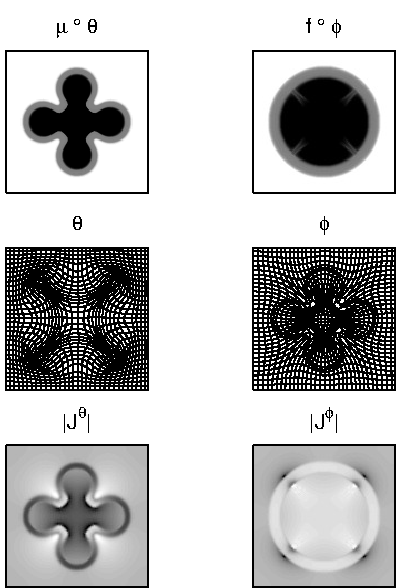
\includegraphics[width=\textwidth]{shoot2d}
\end{columns}
\end{frame}

\begin{frame}
\frametitle{Different ways of measuring distances}
\begin{columns}[c]
\column{.3\textwidth}
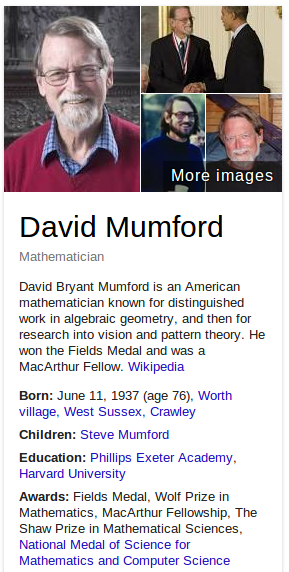
\includegraphics[width=\textwidth]{mumford}
\column{.7\textwidth}
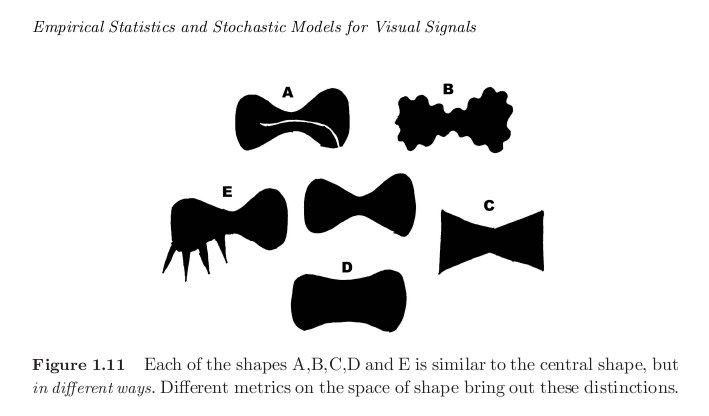
\includegraphics[width=\textwidth]{mumford_fig}
\end{columns}
\end{frame}

\begin{frame}
\frametitle{Different ways of measuring distances}
\begin{columns}[c]
\column{.2\textwidth}
\begin{center}
Two simulated images\par
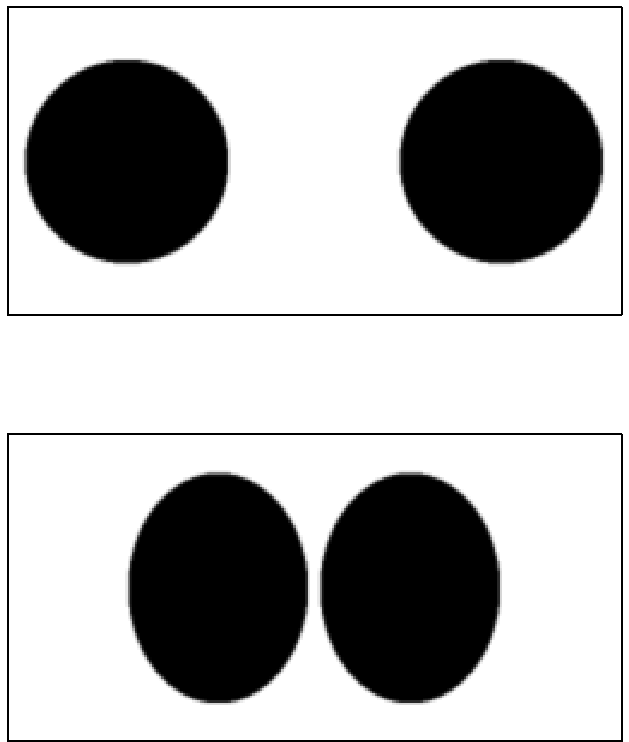
\includegraphics[width=\textwidth]{figure2Di}
\end{center}
\column{.8\textwidth}
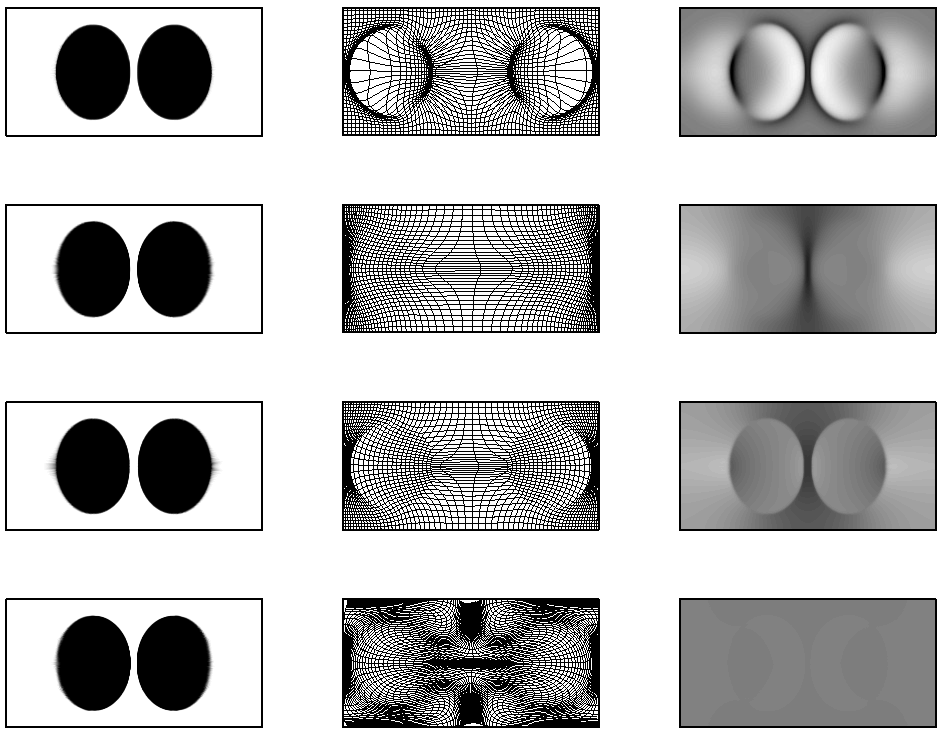
\includegraphics[width=\textwidth]{figure2Dii}
\end{columns}
\end{frame}

\begin{frame}
\frametitle{Metrics}
Distances need to satisfy the properties of a \emph{metric}:
\begin{enumerate}
\item $d({\bf x}, {\bf y}) \ge 0$ (non-negativity)
\item $d({\bf x}, {\bf y}) = 0$ if and only if ${\bf x} = {\bf y}$ (identity of indiscernibles)
\item $d({\bf x}, {\bf y}) = d({\bf y}, {\bf x})$ (symmetry)
\item $d({\bf x}, {\bf z}) \le d({\bf x}, {\bf y}) + d({\bf y}, {\bf z})$ (triangle inequality).
\end{enumerate}

Satisfying (3) requires inverse-consistent image registration.

Satisfying (4) requires a specific class of image registration models.
\end{frame}


\begin{frame}
\frametitle{Non-Euclidean geometry}
\begin{columns}[c]
\column{0.5\textwidth}
\begin{itemize}
\item Distances are not always measured along a straight line.
\item ``\emph{Shapes are the ultimate non-linear sort of thing}''
\end{itemize}
\column{0.5\textwidth}
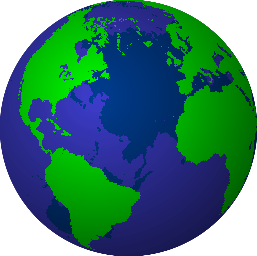
\includegraphics[width=\textwidth]{Globe}
\end{columns}
\end{frame}

\begin{frame}
\frametitle{Linear approximations to nonlinear problems}
%\begin{columns}[c]
%\column{0.2\textwidth}
%Dealing with non-Euclidean geometry.
%Linear approximation around the average.
%\begin{center}
%\column{0.8\textwidth}
\begin{center}
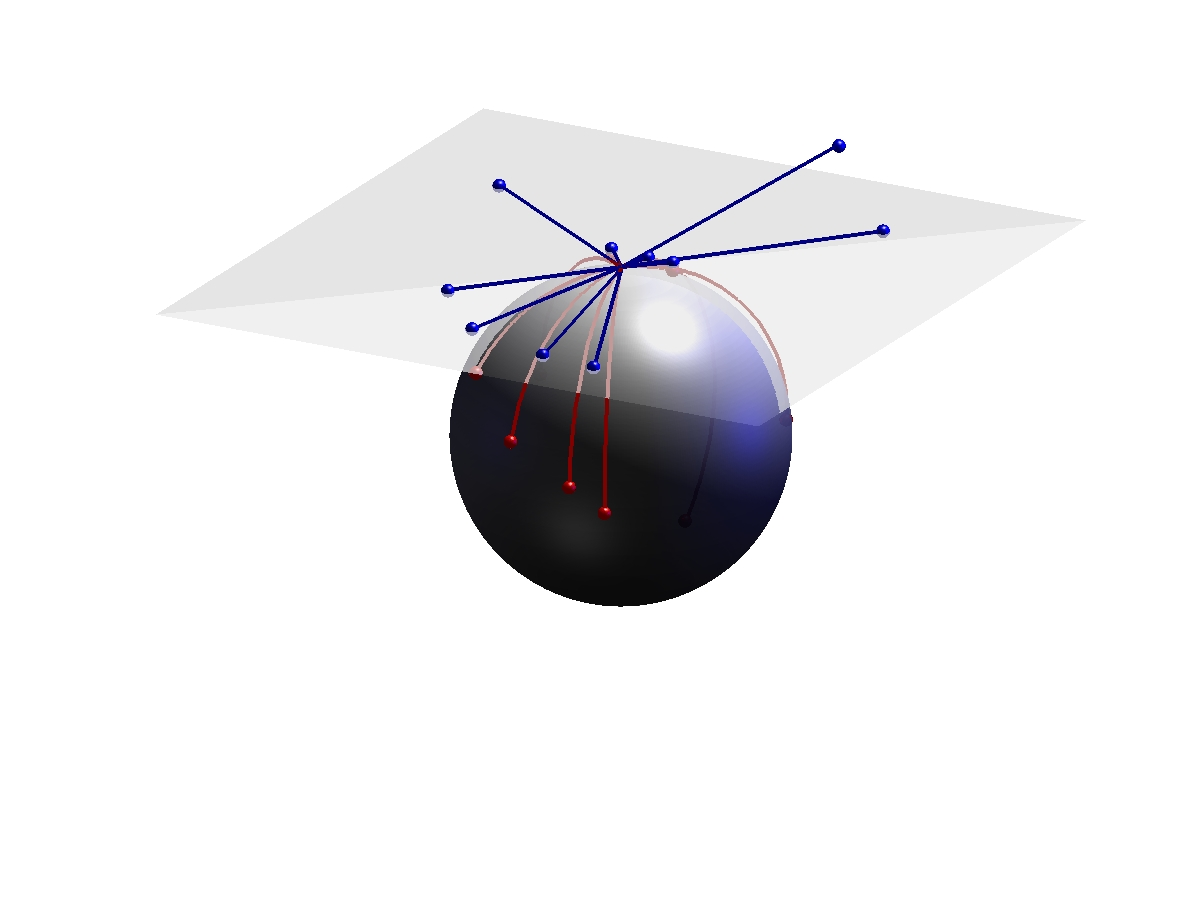
\includegraphics[width=1.2\textwidth]{spheres}
\end{center}
%\end{columns}
\end{frame}

%\begin{frame}
%\frametitle{D'Arcy Thompson's Generative Model}
%\begin{quote}
%``...diverse and dissimilar fishes can be referred as a whole to identical functions of very different co-ordinate systems...''
%\end{quote}
%\begin{center}
%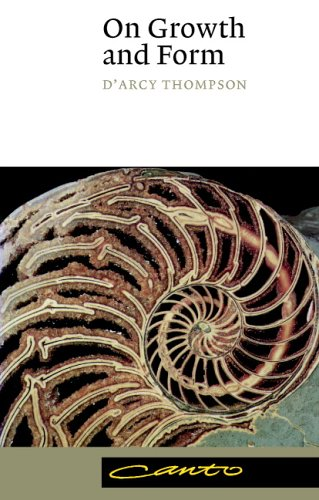
\includegraphics[height=0.4\textheight]{OGAF}
%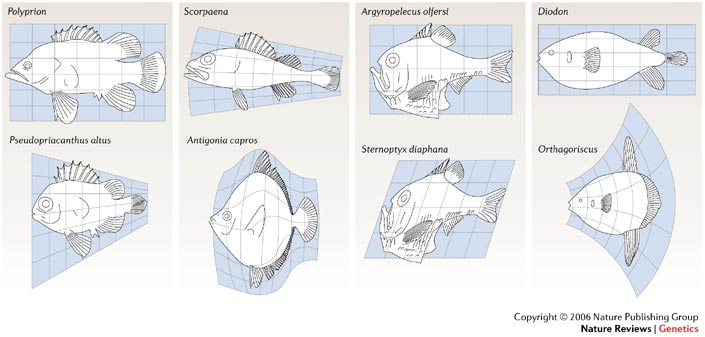
\includegraphics[height=0.4\textheight]{fish}
%\end{center}
%We can compute relative shapes using image registration.
%\end{frame}

